\documentclass{beamer}

\usepackage{subfigure}
\usepackage{graphicx}
\usepackage{sidecap}
\usepackage{caption}
%\usepackage{subcaption}
\captionsetup{compatibility=false}
\usepackage{appendixnumberbeamer}
\usepackage{amsmath}
% --
\usepackage{multirow}
\usepackage{xcolor}
\usepackage{setspace}
\usepackage{hyperref}
\usepackage{anyfontsize}

\setbeamertemplate{footline}

\newenvironment{itemise} {\begin{itemize} \setlength{\itemsep}{0.2cm}} {\end{itemize}}
\usepackage[labelformat=empty]{caption}
\setbeamertemplate{sections/subsections in toc}[square]

%% COLORS
\definecolor{Gray}{gray}{0.9}
\definecolor{dblue}{rgb}{0.132,0.1,0.27}
\definecolor{mint}{cmyk}{1.0, 0.2, 0.6, 0.05}
\definecolor{ant}{cmyk}{0.5, 0.1, 0.0, 0.45}
\definecolor{lgray}{cmyk}{0.12, 0.0, 0.0, 0.17}
\definecolor{lred}{cmyk}{0.0, 0.9, 0.7, 0.0}


\usepackage{etoolbox}% http://ctan.org/pkg/etoolbox 
\usepackage{booktabs}

\newenvironment{literatur}{%
  \parskip2pt \parindent0pt \raggedright
  \def\lititem{\hangindent=0.5cm \hangafter1}}{%
  \par\ignorespaces}

\newcommand{\tb}[1]{{\color{blue}{\textbf{#1}}}}
\newcommand{\tm}[1]{{\color{mint}{\textbf{#1}}}}
\newcommand{\tr}[1]{{\color{red}{\textbf{#1}}}}
% Ilya: packages

\usepackage{tikz}
\usepackage{lmodern}
\usepackage{enumitem}

% Ilya: my commands

\newenvironment{mytemize}
{\vfill\itemize[nolistsep,itemsep=\fill,label=\color{blue}{$\triangleright$}]}
  {\enditemize}


\newenvironment{mynumerate}
{\vfill\enumerate[nolistsep,itemsep=\fill,label=\arabic*.]}
  {\endenumerate}

\newcommand{\hitem}[1]{
  {\color{blue}{$\triangleright$}} 
  {#1} 
  {\hfill}
}

\setlist[itemize]{label= \color{blue}{$\triangleright$}}
\setlist[enumerate]{label = \arabic*.}

\newcommand{\rarr}{$\Rightarrow$\ }



%\href{<Ziel>}{<Eingefasster Text>} 

%\logo{\includegraphics[height=0.7cm]{BdFlogo.eps}\hspace{300pt}\vspace{-5pt}}
%\logo{\includegraphics[height=0.8cm]{BdFlogo.eps}}
%\logo{\pgfputat{\pgfxy(-6.2,-0.5)}{\pgfbox[center,base]{\includegraphics[height=0.8cm]{BdFlogo.eps}}}}

%------------------------------------------------------------------------------------
% TITLE
%------------------------------------------------------------------------------------
\title[PSME]{Macroeconomics\\ Lecture 4 -- Open Economy: IS-TR-IFM, AD-AS } 
\author[I. Eryzhenskiy]{Ilya Eryzhenskiy}
\institute[BdF]{PSME Panth\'{e}on-Sorbonne Master in Economics}
\date[PSME macro]{Fall 2022}

%---BEGIN------------------------------------------------------------------------------
\begin{document}

\begin{frame}
  \maketitle
\end{frame}

\begin{frame}{Overview}
  \tableofcontents
\end{frame}

\section{Exchange rates}

\begin{frame}{Open economy: new market(s)}
  \begin{figure}
	\centering
	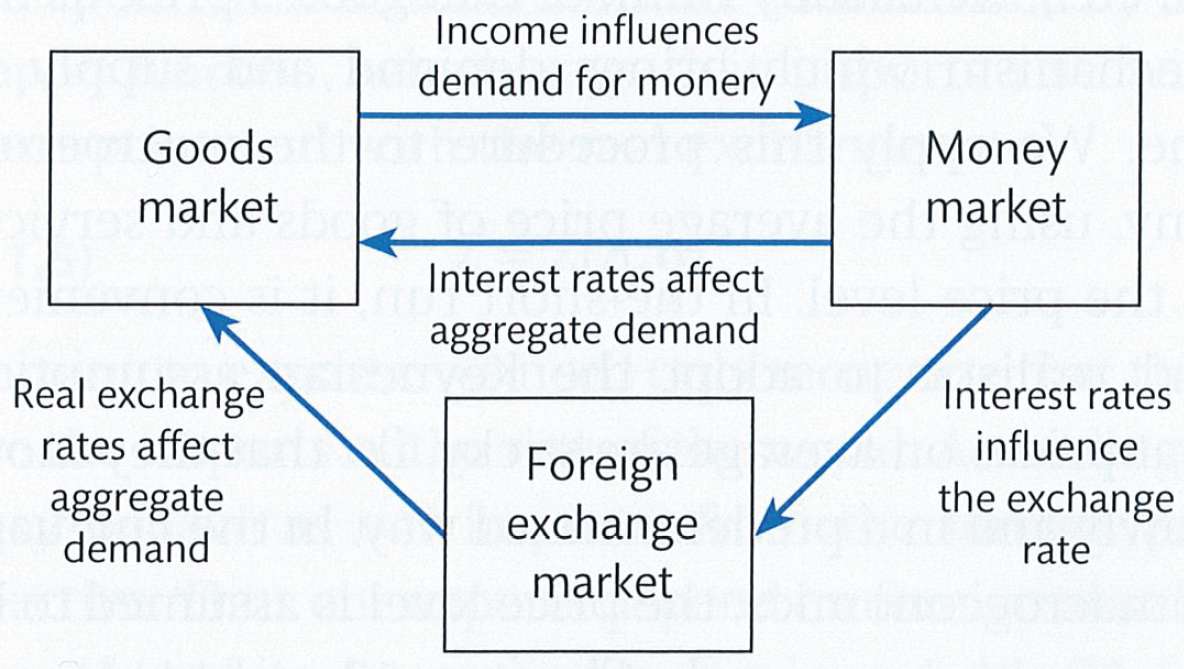
\includegraphics[width=0.8\textwidth]{FIGURES/6_GE.png}
  \end{figure}
\begin{minipage}{1.0\columnwidth}
\tiny	
%	\textbf{Note.} The Figure shows the average behaviour of variables around cyclical peaks in eight countries.\\
\textbf{Source.} Burda and Wyplosz (2017), Figure 10.2.\\
\end{minipage}
\end{frame}

\begin{frame}{%
\protect\hypertarget{lecture-overview-opening-up-is-tr-and-ad-as}{%
Lecture overview: opening up IS-TR and AD-AS}}

\begin{mynumerate}
 
 
\item
  Goods market has imports and exports \rarr IS equation has new terms

  \begin{mytemize}
   
  \item
	\tb{Exchange rate} movements \textbf{shift} IS
  \end{mytemize}
\item
  International financial markets influence nominal interest rate
  \rarr \tb{IFM line}

  \begin{mytemize}
   
  \item
    IS-TR-IFM or Mundell-Flemming model
  \end{mytemize}
\item
  Medium run (AD-AS): inflation affects \tb{real exchange rate} 

\item
  Long run: \tb{purchasing power parity} affects inflation and exchange rate 
\end{mynumerate}
\vfill
Distinction between \tb{fixed} and \tb{flexible} exchange rate regimes.
\vfill
AS is same as in closed economy (simplification).

\end{frame}

\begin{frame}{%
\protect\hypertarget{exchange-rates-quick-overview}{%
Exchange rates -- quick overview}}

\tm{Nominal} vs. \tb{real} exchange rates:

\begin{mytemize}
 
\item
  \tm{Nominal} exchange rate -- number of units of one currency per unit
  of another \(\Leftrightarrow\) \textbf{relative price of monies}

  \begin{mytemize}
   
  \item
    Can be expressed in units of foreign currency per unit of domestic
    or vice versa
  \item
    Example: EUR-JPY exchange rate is 140 JPY for 1 EUR
  \end{mytemize}
\item
  \tb{Real} exchange rate (RER) - ratio of foreign consumption basket value to
  domestic consumption basket value \(\Leftrightarrow\) \textbf{relative
  price of consumption}
\end{mytemize}

Using \(S\) as \tm{nominal} exchange rate (number of units of foreign
currency per unit of domestic), \(P\) the domestic and \(P^*\) the
foreign price level, define the \tb{real} exchange rate \(\sigma\) as:
\[ \sigma = \frac{S \cdot P}{P^*}\]

\end{frame}

\begin{frame}{RER dynamics formula}
  Taking logs and total differential in the real exchange rate definition:
$$\frac{d \sigma}{\sigma} = \frac{d S}{S} + \frac{d P}{P}  - \frac{d P^*}{P^*} $$
$$\frac{d \sigma}{\sigma} = \frac{d S}{S} + \pi  - \pi^* $$
  
\end{frame}

\begin{frame}{Long run real exchange rate}
  Absence of \tb{arbitrage} between countries assumed in long run \rarr two versions of \tb{purchasing power parity (PPP)} condition:
  \begin{mynumerate}
  \item \tb{Absolute PPP}: $\sigma = 1 \Leftrightarrow S \cdot P  = P^*$
  \item \tb{Relative PPP}: $\sigma$ constant: 
	$$d \sigma = 0 \Rightarrow \frac{d \sigma}{\sigma} = \frac{d S}{S} + \frac{d P}{P}  - \frac{d P^*}{P^*} = 0$$
	$$\frac{d S}{S} = \pi^* - \pi$$
  \item[\rarr] if domestic and foreign inflation rates not equal on average, permanent nominal exchange rate appreciation/depreciation
  \end{mynumerate}
  \vfill
  Micro version of PPP -- \tr{law of one price}: each good $j$ has same price in domestic and foreign economy: $S \cdot p_j = p^*_j$ \\ Sufficient, but \textbf{not necessary} for PPP to hold.
\end{frame}

\begin{frame}{Real exchange rate: Example}
  
  \begin{figure}[ht]
	\centering
	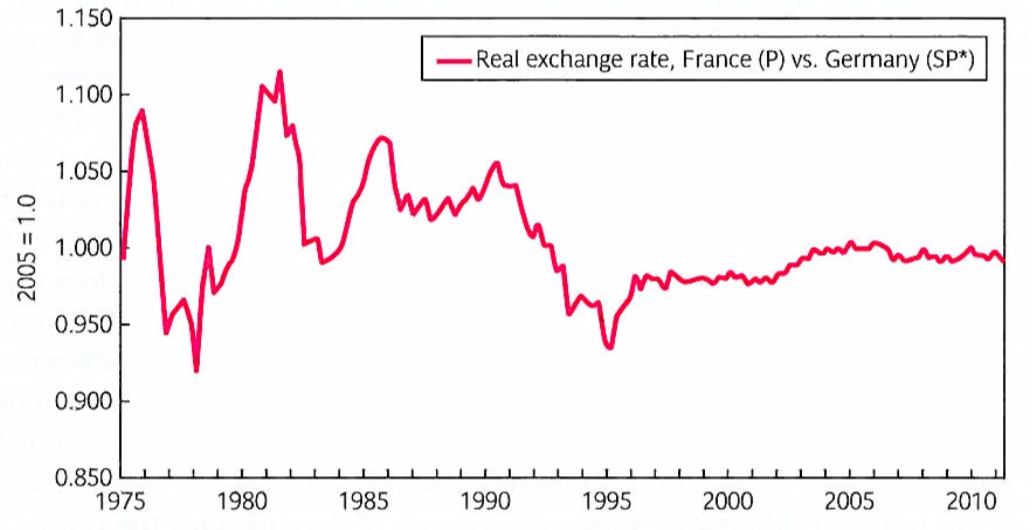
\includegraphics[width=0.95\textwidth]{FIGURES/Fig_13_9_RER_France_Germany}
 \end{figure}
 \begin{minipage}{0.6\columnwidth}
\tiny	
%\textbf{Note.} Actual examples of trajectories, extracted from the French and Italian CPI databases. The dotted lines indicate events of price changes.
\textbf{Source.} Burda and Wyplosz (2017), Figure 13.9.\\
\end{minipage}
\end{frame}


\section{IS in open  economy}
\begin{frame}{IS curve in open economy}

  IS obtained from equality of total goods available (left hand side) and all the uses of the goods (right hand side):
\begin{align*}
  Y + \underbrace{Z}_{\text{imports}}=C+I+G+\underbrace{X}_{\text{exports}} 
\end{align*}
Re-arranging, we get:
\begin{align*}
  Y=C+I+G+\underbrace{(X-Z)}_{\text{primary current account (PCA)}}
\end{align*}
\end{frame}

\begin{frame}{Primary current account}

\tm{Import function}
\begin{equation}
Z = Z(\underset{+}{Y},\underset{+}{\sigma}) \tag{11.5}
\end{equation}
\begin{itemize}
  \item Increases in income (proportional to disposable income or to consumption), example: $Z = z \cdot C = z \cdot c \cdot (Y-T))$
\item Increases with real exchange rate appreciation ($\sigma \uparrow$, where $\sigma=SP/P^*$), domestic goods relatively expensive \rarr import$\uparrow$
\end{itemize}

\tm{Export function}
\begin{equation}
X = X(\underset{+}{Y^*},\underset{-}{\sigma}) \tag{11.6}
\end{equation}
\begin{itemize}
  \item \textbf{demand-driven exports}: foreign income $\Rightarrow$ foreign demand. Domestic income/production not relevant!
\item with real exchange rate appreciation ($\sigma \uparrow$), domestic goods relatively expensive \rarr less exports
\end{itemize}

\tb{Primary Current Account (PCA)} or Net Exports:
\begin{align*}
PCA = &X(\underset{+}{Y^*},\underset{-}{\sigma})-Z(\underset{+}{Y},\underset{+}{\sigma}) \\
 =	 & PCA(\underset{-}{Y},\underset{+}{Y^*},\underset{-}{\sigma})   
\end{align*}

\end{frame}

\begin{frame}{Keynesian multiplier in open economy}
  Assume linear functions: $C = c\cdot (Y-T)$ \\ $Z = z\cdot C = z \cdot c \cdot (Y-T)$ \\
Consider an increase in government expenditure, $\Delta G$
\begin{itemize}
\small
\item $DD\uparrow$, firms will produce more, ..., $Y\uparrow$
\item \tb{Multiplier}: how much output changes $\Delta Y$, relative to shock $\Delta G$
\item firms will increase production by $\Delta G$
\item this generates new income, thus $C\uparrow$ but $PCA\downarrow$, $\Delta DD = c \Delta G - z c \Delta G = c(1-z)\Delta G$
\item[$\rightarrow$] $Y\uparrow, C\uparrow, PCA\uparrow, Y\uparrow\dots$ -- recall staircase graph
\item additional spending $\Delta C + \Delta PCA$ is smaller than $\Delta G$ due to \textit{leakages}, so $\Delta Y_2< \Delta Y_1$
\item leakages in open economy: savings, \tr{imports}, taxes (if proportional)
%\item $\Delta Y/\Delta G >1$
\end{itemize}
{
\begin{align*}
\Delta Y =& \Delta G + c(1-z)\Delta G + c^2(1-z)^2\Delta G + ...+c^n(1-z)^n\Delta G \\
	&= \underbrace{\alert{\frac{1}{1-c(1-z)}}}_{\text{multiplier}>1} \Delta G
\end{align*}
}
\end{frame}


%---FRAME------------------------------------------------------------------------------
\begin{frame}{Open economy IS}
 Key question: how change of real exchange rate $\sigma$ affect IS?
 \begin{mytemize}
\item RER appreciation \rarr more imports, less exports \rarr for a given interest rate, goods market equilibrium has lower $Y$ because of lower aggregate demand
 \end{mytemize}
\begin{align*}
Y = C(\underset{+}{\Omega}, \underset{+}{Y-T}) + I(\underset{-}{r}, \underset{+}{q}) + G + PCA(\underset{-}{Y},\underset{+}{Y^*},\underset{-}{\sigma})
\end{align*}
\begin{align*}
  \underbrace{Y - C(\Omega, Y-T) -  PCA(Y,Y^*,\sigma)}_{\text{increases in}\ Y,\ \sigma}=  I(\underset{-}{i - \pi^e}, q) + G 
\end{align*}
\begin{mytemize}
\item Mathematics: left hand side increasing in both $Y$ and $\sigma$ \rarr for a fixed right hand side, $Y\downarrow$ when $\sigma\uparrow$ for equation to hold
\item[\rarr] when $\sigma\uparrow$, $Y\downarrow$ for fixed $i$ \rarr \tr{IS moves left} in $(Y, i)$ space. 
\end{mytemize}
\end{frame}

\section{Capital flows: IFM line}
\begin{frame}{What are capital flows?}
  This lecture: wider notion of capital, including any assets $+$ currency. \\
  \vfill
  Any purchase/sale of foreign assets is registered in country's international capital flows.
Examples: 
\begin{mytemize}
\item Use of foreign currency
\item Lending/borrowing with non-resident
\item Foreign direct investment
\end{mytemize}
\vfill
Policy of capital movement restriction: \tr{capital controls}
\begin{mytemize}
\item Goes against orthodox economic theory/finance, but\dots
\item Actively used by China \rarr relevant for understanding world economy
\item \tr{Not studied} in this lecture
\end{mytemize}
\end{frame}

\begin{frame}{International financial market: capital flows}
  
  We adopt assumption of \tb{small open economy} with free capital flows (no \tr{capital controls}):
  \begin{mytemize}
  \item Recall small open economy definition: country does not influence international prices
  \item \dots in particular, international nominal interest, $i^*$
  \item free capital flows \rarr no \tb{arbitrage} possibilities between domestic and foreign assets, \textbf{returns are equalized}: $i = i^*$
  \item[\rarr] a new condition in the $(Y, i)$ space: a horizontal IFM line
  \end{mytemize}
\end{frame}

\begin{frame}{Economy off IFM line -- exchange rate regime matters}
  What happens after capital inflows/outflows? What consequences for IS, TR \rarr for AD?
  \vfill
  $\rightarrow$ answers depend on \tb{exchange rate regime}
  \begin{mytemize}
  \item Under \tb{fixed exchange rate regime}, CB must prevent changes in \tm{nominal exchange rate}
	\begin{mytemize}
	\item Taylor Rule, money supply change such that $i = i^*$ again
	\end{mytemize}
  \item  Under \tb{flexible exchange rate regime}, CB does not react, nominal exchange rate changes, IS shifts 
	\begin{mytemize}
	\item Additional stability of IS following demand shocks
	\end{mytemize}
  \end{mytemize}
\end{frame}

\section{Fixed exchange rate regime}
\begin{frame}
\tableofcontents[currentsection]
\end{frame}

\subsection{IS-(TR)-IFM equilibrium}
\begin{frame}{%
\protect\hypertarget{fixed-exchange-rate-in-is-tr}{%
Fixed exchange rate in IS-TR}}

\begin{mytemize}

\item
  Open economy \rarr loss of monetary autonomy because of capital flows:
  i = i*
\item
  Choice of money supply by the CB dictated by exchange rate
\item
  Taylor Rule is no longer determining equilibrium
\item
  The horizontal IFM line in (i, Y) space determines equilibrium instead
  of TR 
\end{mytemize}
\vfill  We will consider different types of shocks in this IS-(TR)-IFM
  framework.
\end{frame}

\begin{frame}{%
\protect\hypertarget{demand-shock-e.g.government-spending}{%
Demand shock (e.g.~government spending)}}

\end{frame}


\begin{frame}{%
\protect\hypertarget{devaluationsrevaluations-a-monetary-policy-shock}{%
Devaluations/revaluations -- monetary policy via $\bar S$}}

\end{frame}

\begin{frame}{%
\protect\hypertarget{devaluationsrevaluations-a-monetary-policy-shock}{%
Devaluations/revaluations -- monetary policy via $\bar S$}}

\begin{mytemize}

\item
  IS moves as explored before
\item
  Central bank must adapt monetary policy -- TR shifts
\item
  Behind the scenes -- central bank buys or sells foreign currency to
  keep S fixed -- \tb{foreign exchange interventions}
\item
  Change of CB \textbf{assets} must be coupled with changes of
  \textbf{liabilities} -- the money supply
\item
  Process known as \tb{sterilisation} of foreign exchange interventions
\end{mytemize}

\end{frame}

\begin{frame}{%
\protect\hypertarget{international-financial-shock-shift-of-ifm}{%
International financial shock -- shift of IFM}}

\begin{columns}
\column{0.35\textwidth}
An increase in world interest rate is contractionary for fixed exchange rate economies\\
\vspace{3cm}
Relevant shock for 2022!
\column{0.65\textwidth}
\end{columns}

\end{frame}

\subsection{AD-AS}

\begin{frame}{LAD under fixed exchange rates: Purchasing Power Parity}
  Absence of \tb{arbitrage} between countries assumed in long run \rarr two versions of \tb{purchasing power parity (PPP)} condition:
  \begin{mynumerate}
  \item \tb{Absolute PPP}: $\sigma = 1 \Leftrightarrow S \cdot P  = P^*$
  \item \tb{Relative PPP}: $\sigma$ constant: 
	$$d \sigma = 0 \Rightarrow \frac{d \sigma}{\sigma} = \underbrace{\frac{d S}{S}}_{=0} + \pi  - \pi^* = 0 \Leftrightarrow \pi = \pi^*$$
  \item[\ ] Relative PPP follows from absolute, so it is always assumed.
  \item[\rarr] domestic inflation rate must equal foreign in long run -- horizontal long-run aggregate demand line (LAD) at $\pi = \pi^*$
  \end{mynumerate}
  %\vfill
  %Most strict version -- \tr{law of one price}: each good $j$ has same price in domestic and foreign economy: $S \cdot p_j = p^*_j$ -- sufficient, but \textbf{not necessary} for PPP to hold.
\end{frame}

\begin{frame}{Medium-run AD under fixed exchange rate}
\begin{columns}
\column{0.5\linewidth}
\begin{itemize}
\item Assuming $\pi\uparrow$
\item $\frac{d \sigma}{\sigma} = \frac{d S}{S} + \pi  - \pi^* = \pi - \pi^*$ \rarr $\sigma\uparrow$
\item IS-(TR)-IFM: IS shifts to the left, intersection with IFM has lower $Y$
\item[\rarr] inflation higher, output lower: downward sloping medium run \emph{AD curve}
\end{itemize}
\textbf{Shifts in AD}
\begin{itemize}
  \item Demand shocks (incl. $Y^*$)
  \item Devaluations, revaluations ($\bar S$)
  \item IFM ($i^*$) 
\end{itemize}
% COLUMN(2)
\column{0.45\linewidth}

\centering
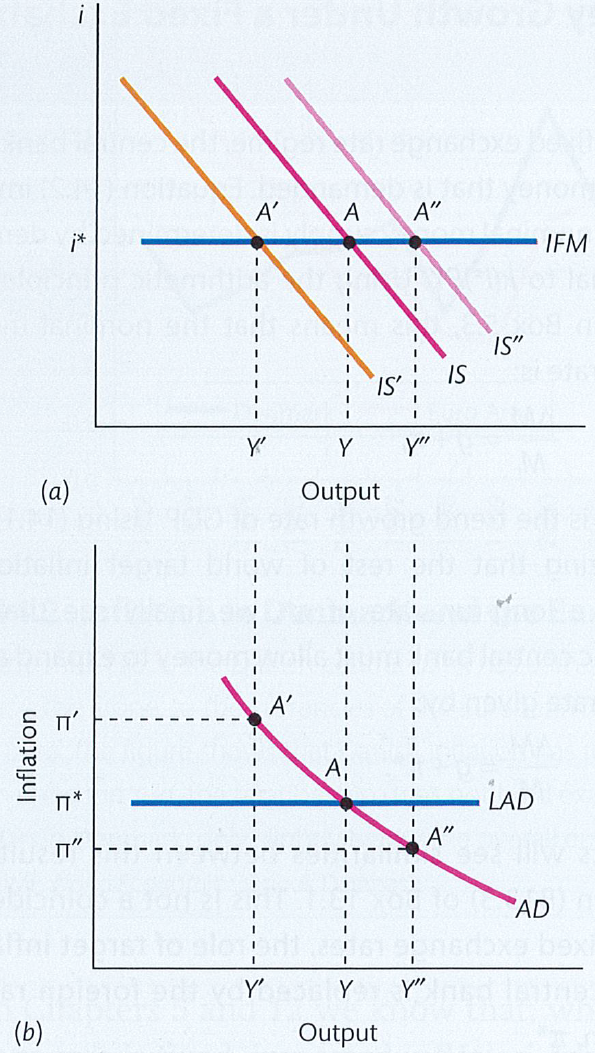
\includegraphics[clip,width=1\columnwidth]{FIGURES/9_AD_FixedFX}
%\vspace{-2mm}

\begin{minipage}{1.0\columnwidth}
\tiny	
%	\textbf{Note.} The Figure shows the average behaviour of variables around cyclical peaks in eight countries.\\
\textbf{Source.} Burda and Wyplosz (2017), Figure 14.11.\\
\end{minipage}
	
\end{columns} 	 
\end{frame}

\begin{frame}{AD-AS with fixed exchange rate regime}
  \vspace{-5cm}
  New mechanism: long-run convergence of $\pi$ to $\pi^*$ through changes of $\sigma$.
\end{frame}

\section{Flexible exchange rate regime}
\begin{frame}
\tableofcontents[currentsection]
\end{frame}
\subsection{(IS)-TR-IFM equilibrium}
\subsection{AD-AS}
\begin{frame}{%
\protect\hypertarget{flexible-exchange-rate}{%
Flexible exchange rate}}

\begin{mytemize}
 
\item
  Monetary policy is again independent
\item
  Aggregate demand has additional source of variation: RER changes through \tb{nominal interest rate}
\item Position of IS becomes endogenous as TR and IFM determine equilibrium: (IS)-TR-IFM
\end{mytemize}

\end{frame}

\begin{frame}{%
\protect\hypertarget{monetary-policy-shock-graph}{%
Monetary policy shock with flexible exchange rates}}
\vspace{-5cm}
Monetary policy \textit{de facto} operates through \tr{exchange rate} and \tr{not interest rate}

\end{frame}

\begin{frame}{%
\protect\hypertarget{demand-shock-e.g.government-spending}{%
Demand shock (e.g.~government spending) with flexible exchange rates}}
\vspace{-5cm}
Exchange rate acts as \tr{stabilizer} of aggregate demand
 

\end{frame}

\begin{frame}{%
\protect\hypertarget{international-monetary-shock}{%
International monetary shock}}
\vspace{-5cm}
An increase in foreign interest rate is \tr{expansionary} --\\
\tr{opposite} of \tr{fixed} exchange rate case.

\end{frame}

\begin{frame}{%
\protect\hypertarget{international-monetary-shock-ii-beggar-thy-neighbour-effect}{%
International monetary shock II: beggar-thy-neighbour effect}}

\begin{mytemize}
 
\item
  Suppose a large foreign economy lowers $i^*$ in expansionary monetary
  policy
\item
  What happens to domestic economy? Draw an (IS)-TR-IFM diagram!
\item
  Domestic $i$ relatively high \rarr capital inflow \rarr real exchange
  rate appreciation \(\sigma \uparrow\)
\item
  IS moves to the left, equilibrium output lower
\item
  Foreign expansionary policy at the expense of neighbours' output. A critique of expansionary QE policies in large Western economies post-2008, from smaller economies' perspective.
\end{mytemize}

\end{frame}

\begin{frame}{%
\protect\hypertarget{flexible-exchange-rate-ad}{%
LAD under flexible exchange rate}}

\begin{mytemize}
 
\item
  LAD: Taylor rule enforces \(\pi = \bar \pi\) in long run, as in closed economy
  \item \tr{Different} from \tr{fixed} exchange rate regime, where LAD is $\pi = \pi^*$
\end{mytemize}

\end{frame}

\begin{frame}{Medium-run AD under flexible exchange rate regime}
\begin{columns}
\column{0.5\linewidth}
\begin{itemize}
\item Assuming $\pi\uparrow$
\item $\frac{d \sigma}{\sigma} = \frac{d S}{S} + \pi  - \pi^*$ \rarr $\sigma\uparrow$
\item IS shifts to the left, TR shifts up -- IS-TR-IFM intersection with lower $Y$
\item[\rarr] inflation higher, output lower: downward sloping medium run AD curve
\end{itemize}
\textbf{Shifts in AD}
\begin{itemize}
  \item \tr{NOT} the demand shocks (IS shifters other than $\sigma$) 
  \item TR shocks ($\bar i, \bar \pi$)
  \item IFM ($i^*$) -- opposite effect to fixed exchange rate case
\end{itemize}
% COLUMN(2)
\column{0.45\linewidth}

\centering
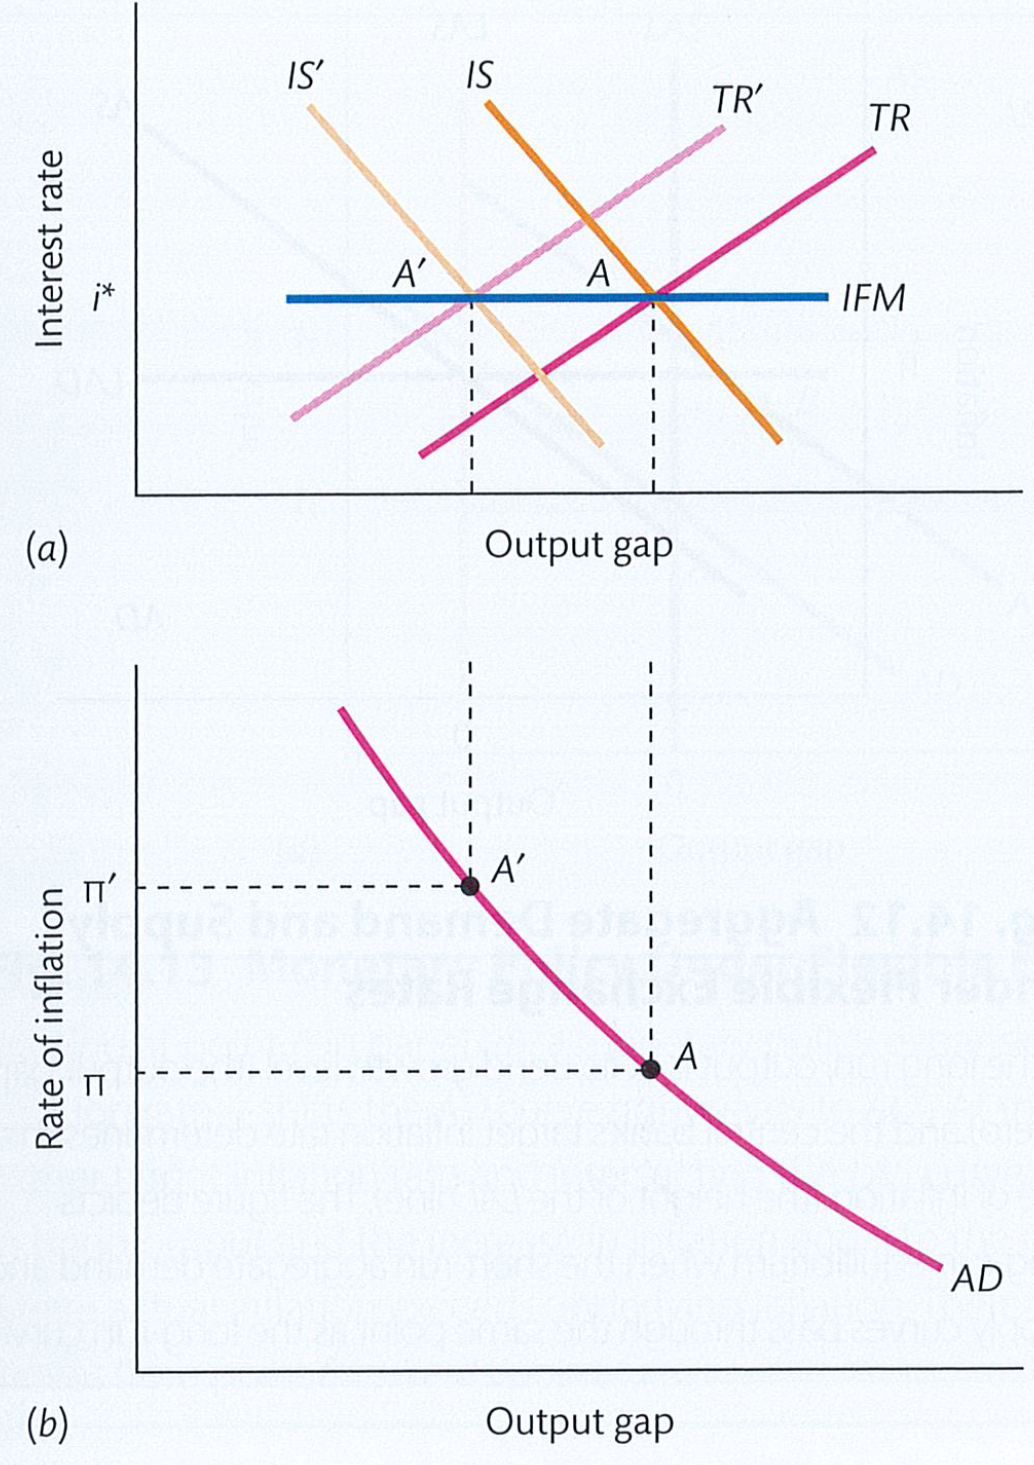
\includegraphics[clip,width=1\columnwidth]{FIGURES/9_ASAD_Flexible_shortrun.png}
%\vspace{-2mm}

\begin{minipage}{1.0\columnwidth}
\tiny	
%	\textbf{Note.} The Figure shows the average behaviour of variables around cyclical peaks in eight countries.\\
\textbf{Source.} Burda and Wyplosz (2017), Figure 14.11.\\
\end{minipage}
	
\end{columns} 	 
\end{frame}

\begin{frame}{AD-AS under flexible exchange rate regime}
  \vspace{-5cm}
  Similar to closed economy, with additional shifts in AD due to $\sigma$.
\end{frame}

\section{More on exchange rate regimes}
\begin{frame}
\tableofcontents[currentsection]
\end{frame}

\begin{frame}{Recap: trade-offs of exchange rate regimes}
  Each exchange rate regime presents pros and cons. Seen in this lecture: 
  \begin{mytemize}
  \item \tb{Fixed} exchange rate regime:
	\begin{mytemize}
	\item  facilitates trade of goods, services and assets, \tr{but}
	\item eliminates independent monetary policy (control over $i$)
	\item not necessarily bad, e.g. if CB has \tb{commitment} problems leading to high inflation
	\end{mytemize}
  \item \tb{Flexible} of floating exchange rate regime:
	\begin{mytemize}
	\item creates problems in trade, \tr{but}
	\item allows for monetary policy $+$ acts as absorber of demand shocks
	\end{mytemize}
  \end{mytemize}
  Important issues of \tb{foreign exchange reserves} management not covered in lecture -- another argument against fixed regimes when CB is not trusted by public.
\end{frame}

\begin{frame}{Beyond fixed vs. flexible: IMF classification}
  Many regimes exist as countries trade off benefits and costs of fixed and flexible exchange rates.
  \begin{figure}[ht]
	\centering
	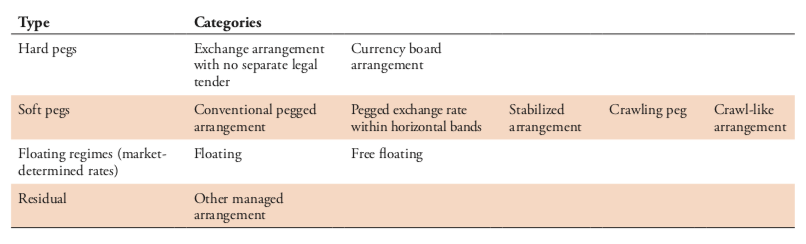
\includegraphics[width = 1.1\textwidth]{FIGURES/IMF_exchange_rate_regimes}
  \end{figure}
	\tiny Source: IMF Annual report on exchange arrangements and exchange restrictions (2021).
\end{frame}

\end{document}
